% uWaterloo Thesis Template for LaTeX 
% Last Updated June 14, 2017 by Stephen Carr, IST Client Services
% FOR ASSISTANCE, please send mail to rt-IST-CSmathsci@ist.uwaterloo.ca

% Effective October 2006, the University of Waterloo 
% requires electronic thesis submission. See the uWaterloo thesis regulations at
% https://uwaterloo.ca/graduate-studies/thesis.

% DON'T FORGET TO ADD YOUR OWN NAME AND TITLE in the "hyperref" package
% configuration below. THIS INFORMATION GETS EMBEDDED IN THE PDF FINAL PDF DOCUMENT.
% You can view the information if you view Properties of the PDF document.

% Many faculties/departments also require one or more printed
% copies. This template attempts to satisfy both types of output. 
% It is based on the standard "book" document class which provides all necessary 
% sectioning structures and allows multi-part theses.

% DISCLAIMER
% To the best of our knowledge, this template satisfies the current uWaterloo requirements.
% However, it is your responsibility to assure that you have met all 
% requirements of the University and your particular department.
% Many thanks for the feedback from many graduates that assisted the development of this template.

% -----------------------------------------------------------------------

% By default, output is produced that is geared toward generating a PDF 
% version optimized for viewing on an electronic display, including 
% hyperlinks within the PDF.
 
% E.g. to process a thesis called "mythesis.tex" based on this template, run:

% pdflatex mythesis	-- first pass of the pdflatex processor
% bibtex mythesis	-- generates bibliography from .bib data file(s)
% makeindex         -- should be run only if an index is used 
% pdflatex mythesis	-- fixes numbering in cross-references, bibliographic references, glossaries, index, etc.
% pdflatex mythesis	-- fixes numbering in cross-references, bibliographic references, glossaries, index, etc.

% If you use the recommended LaTeX editor, Texmaker, you would open the mythesis.tex
% file, then click the PDFLaTeX button. Then run BibTeX (under the Tools menu).
% Then click the PDFLaTeX button two more times. If you have an index as well,
% you'll need to run MakeIndex from the Tools menu as well, before running pdflatex
% the last two times.

% N.B. The "pdftex" program allows graphics in the following formats to be
% included with the "\includegraphics" command: PNG, PDF, JPEG, TIFF
% Tip 1: Generate your figures and photos in the size you want them to appear
% in your thesis, rather than scaling them with \includegraphics options.
% Tip 2: Any drawings you do should be in scalable vector graphic formats:
% SVG, PNG, WMF, EPS and then converted to PNG or PDF, so they are scalable in
% the final PDF as well.
% Tip 3: Photographs should be cropped and compressed so as not to be too large.

% To create a PDF output that is optimized for double-sided printing: 
%
% 1) comment-out the \documentclass statement in the preamble below, and
% un-comment the second \documentclass line.
%
% 2) change the value assigned below to the boolean variable
% "PrintVersion" from "false" to "true".

% --------------------- Start of Document Preamble -----------------------

% Specify the document class, default style attributes, and page dimensions
% For hyperlinked PDF, suitable for viewing on a computer, use this:
\documentclass[letterpaper,12pt,titlepage,oneside,final]{book}
 
% For PDF, suitable for double-sided printing, change the PrintVersion variable below
% to "true" and use this \documentclass line instead of the one above:
%\documentclass[letterpaper,12pt,titlepage,openright,twoside,final]{book}

% Some LaTeX commands I define for my own nomenclature.
% If you have to, it's better to change nomenclature once here than in a 
% million places throughout your thesis!
\newcommand{\package}[1]{\textbf{#1}} % package names in bold text
\newcommand{\cmmd}[1]{\textbackslash\texttt{#1}} % command name in tt font 
\newcommand{\href}[1]{#1} % does nothing, but defines the command so the
\newcommand{\rmx}{\mathrm x}
\newcommand{\imgsrc}[1]{\caption*{\scriptsize{Source: #1}}}

% print-optimized version will ignore \href tags (redefined by hyperref pkg).
%\newcommand{\texorpdfstring}[2]{#1} % does nothing, but defines the command
% Anything defined here may be redefined by packages added below...

% This package allows if-then-else control structures.
\usepackage{ifthen}
\newboolean{PrintVersion}
\setboolean{PrintVersion}{false} 
% CHANGE THIS VALUE TO "true" as necessary, to improve printed results for hard copies
% by overriding some options of the hyperref package below.

%\usepackage{nomencl} % For a nomenclature (optional; available from ctan.org)
\usepackage{amsmath,amssymb,amstext} % Lots of math symbols and environments
\usepackage[pdftex]{graphicx} % For including graphics N.B. pdftex graphics driver 
\usepackage{natbib} % For better bibliography formatting
\usepackage[dvipsnames]{xcolor} % Additional colors
\usepackage{multirow}
\usepackage{bm}
\usepackage{todonotes}
\usepackage{caption}
\usepackage[hyphens]{url}

% Hyperlinks make it very easy to navigate an electronic document.
% In addition, this is where you should specify the thesis title
% and author as they appear in the properties of the PDF document.
% Use the "hyperref" package 
% N.B. HYPERREF MUST BE THE LAST PACKAGE LOADED; ADD ADDITIONAL PKGS ABOVE
\usepackage[pdftex,pagebackref=false]{hyperref} % with basic options
		% N.B. pagebackref=true provides links back from the References to the body text. This can cause trouble for printing.
\hypersetup{
    plainpages=false,       % needed if Roman numbers in frontpages
    unicode=false,          % non-Latin characters in Acrobat’s bookmarks
    pdftoolbar=true,        % show Acrobat’s toolbar?
    pdfmenubar=true,        % show Acrobat’s menu?
    pdffitwindow=false,     % window fit to page when opened
    pdfstartview={FitH},    % fits the width of the page to the window
    pdftitle={Stylistic\ Variation\ in\ Linguistics\ using\ Disentangled\ Latent\ Spaces},    % title: CHANGE THIS TEXT!
    pdfauthor={Vineet John},    % author: CHANGE THIS TEXT! and uncomment this line
    pdfsubject={Natural Language Processing},  % subject: CHANGE THIS TEXT! and uncomment this line
   	pdfkeywords={nlp} {deep-learning} {linguistic}, % list of keywords, and uncomment this line if desired
    pdfnewwindow=true,      % links in new window
    colorlinks=true,        % false: boxed links; true: colored links
    linkcolor=blue,         % color of internal links
    citecolor=red,        % color of links to bibliography
    filecolor=magenta,      % color of file links
    urlcolor=cyan           % color of external links
}
\ifthenelse{\boolean{PrintVersion}}{   % for improved print quality, change some hyperref options
\hypersetup{	% override some previously defined hyperref options
%    colorlinks,%
    citecolor=black,%
    filecolor=black,%
    linkcolor=black,%
    urlcolor=black}
}{} % end of ifthenelse (no else)

\usepackage[automake,toc,abbreviations]{glossaries-extra} % Exception to the rule of hyperref being the last add-on package
% If glossaries-extra is not in your LaTeX distribution, get it from CTAN (http://ctan.org/pkg/glossaries-extra), 
% although it's supposed to be in both the TeX Live and MikTeX distributions. There are also documentation and 
% installation instructions there.

% Setting up the page margins...
% uWaterloo thesis requirements specify a minimum of 1 inch (72pt) margin at the
% top, bottom, and outside page edges and a 1.125 in. (81pt) gutter
% margin (on binding side). While this is not an issue for electronic
% viewing, a PDF may be printed, and so we have the same page layout for
% both printed and electronic versions, we leave the gutter margin in.
% Set margins to minimum permitted by uWaterloo thesis regulations:
\setlength{\marginparwidth}{0pt} % width of margin notes
% N.B. If margin notes are used, you must adjust \textwidth, \marginparwidth
% and \marginparsep so that the space left between the margin notes and page
% edge is less than 15 mm (0.6 in.)
\setlength{\marginparsep}{0pt} % width of space between body text and margin notes
\setlength{\evensidemargin}{0.125in} % Adds 1/8 in. to binding side of all 
% even-numbered pages when the "twoside" printing option is selected
\setlength{\oddsidemargin}{0.125in} % Adds 1/8 in. to the left of all pages
% when "oneside" printing is selected, and to the left of all odd-numbered
% pages when "twoside" printing is selected
\setlength{\textwidth}{6.375in} % assuming US letter paper (8.5 in. x 11 in.) and 
% side margins as above
\raggedbottom

% The following statement specifies the amount of space between
% paragraphs. Other reasonable specifications are \bigskipamount and \smallskipamount.
\setlength{\parskip}{\medskipamount}

% The following statement controls the line spacing.  The default
% spacing corresponds to good typographic conventions and only slight
% changes (e.g., perhaps "1.2"), if any, should be made.
\renewcommand{\baselinestretch}{1} % this is the default line space setting

% By default, each chapter will start on a recto (right-hand side)
% page.  We also force each section of the front pages to start on 
% a recto page by inserting \cleardoublepage commands.
% In many cases, this will require that the verso page be
% blank and, while it should be counted, a page number should not be
% printed.  The following statements ensure a page number is not
% printed on an otherwise blank verso page.
\let\origdoublepage\cleardoublepage
\newcommand{\clearemptydoublepage}{%
  \clearpage{\pagestyle{empty}\origdoublepage}}
\let\cleardoublepage\clearemptydoublepage

% Define Glossary terms (This is properly done here, in the preamble. Could be \input{} from a file...)
% Main glossary entries -- definitions of relevant terminology
 
\makeglossaries

%======================================================================
%   L O G I C A L    D O C U M E N T -- the content of your thesis
%======================================================================
\begin{document}

% For a large document, it is a good idea to divide your thesis
% into several files, each one containing one chapter.
% To illustrate this idea, the "front pages" (i.e., title page,
% declaration, borrowers' page, abstract, acknowledgements,
% dedication, table of contents, list of tables, list of figures,
% nomenclature) are contained within the file "uw-ethesis-frontpgs.tex" which is
% included into the document by the following statement.
%----------------------------------------------------------------------
% FRONT MATERIAL
%----------------------------------------------------------------------
% T I T L E   P A G E
% -------------------
% Last updated June 14, 2017, by Stephen Carr, IST-Client Services
% The title page is counted as page `i' but we need to suppress the
% page number. Also, we don't want any headers or footers.
\pagestyle{empty}
\pagenumbering{roman}

% The contents of the title page are specified in the "titlepage"
% environment.
\begin{titlepage}
        \begin{center}
        \vspace*{1.0cm}

        \Huge
        {\bf University of Waterloo E-Thesis Template for \LaTeX }

        \vspace*{1.0cm}

        \normalsize
        by \\

        \vspace*{1.0cm}

        \Large
        Pat Neugraad \\

        \vspace*{3.0cm}

        \normalsize
        A thesis \\
        presented to the University of Waterloo \\ 
        in fulfillment of the \\
        thesis requirement for the degree of \\
        Doctor of Philosophy \\
        in \\
        Zoology \\

        \vspace*{2.0cm}

        Waterloo, Ontario, Canada, 2017 \\

        \vspace*{1.0cm}

        \copyright\ Pat Neugraad 2017 \\
        \end{center}
\end{titlepage}

% The rest of the front pages should contain no headers and be numbered using Roman numerals starting with `ii'
\pagestyle{plain}
\setcounter{page}{2}

\cleardoublepage % Ends the current page and causes all figures and tables that have so far appeared in the input to be printed.
% In a two-sided printing style, it also makes the next page a right-hand (odd-numbered) page, producing a blank page if necessary.

 
% E X A M I N I N G   C O M M I T T E E (Required for Ph.D. theses only)
% Remove or comment out the lines below to remove this page
\begin{center}\textbf{Examining Committee Membership}\end{center}
  \noindent
The following served on the Examining Committee for this thesis. The decision of the Examining Committee is by majority vote.
  \bigskip
  
  \noindent
\begin{tabbing}
Internal-External Member: \=  \kill % using longest text to define tab length
External Examiner: \>  Bruce Bruce \\ 
\> Professor, Dept. of Philosophy of Zoology, University of Wallamaloo \\
\end{tabbing} 
  \bigskip
  
  \noindent
\begin{tabbing}
Internal-External Member: \=  \kill % using longest text to define tab length
Supervisor(s): \> Doris Johnson \\
\> Professor, Dept. of Zoology, University of Waterloo \\
\> Andrea Anaconda \\
\> Professor Emeritus, Dept. of Zoology, University of Waterloo \\
\end{tabbing}
  \bigskip
  
  \noindent
  \begin{tabbing}
Internal-External Member: \=  \kill % using longest text to define tab length
Internal Member: \> Pamela Python \\
\> Professor, Dept. of Zoology, University of Waterloo \\
\end{tabbing}
  \bigskip
  
  \noindent
\begin{tabbing}
Internal-External Member: \=  \kill % using longest text to define tab length
Internal-External Member: \> Deepa Thotta \\
\> Professor, Dept. of Philosophy, University of Waterloo \\
\end{tabbing}
  \bigskip
  
  \noindent
\begin{tabbing}
Internal-External Member: \=  \kill % using longest text to define tab length
Other Member(s): \> Leeping Fang \\
\> Professor, Dept. of Fine Art, University of Waterloo \\
\end{tabbing}

\cleardoublepage

% D E C L A R A T I O N   P A G E
% -------------------------------
  % The following is a sample Delaration Page as provided by the GSO
  % December 13th, 2006.  It is designed for an electronic thesis.
  \noindent
I hereby declare that I am the sole author of this thesis. This is a true copy of the thesis, including any required final revisions, as accepted by my examiners.

  \bigskip
  
  \noindent
I understand that my thesis may be made electronically available to the public.

\cleardoublepage

% A B S T R A C T
% ---------------

\begin{center}\textbf{Abstract}\end{center}

This is the abstract.

Vulputate minim vel consequat praesent at vel iusto et, ex delenit, esse euismod luptatum augue ut sit et eu vel augue autem feugiat, quis ad dolore. Nulla vel, laoreet lobortis te commodo elit qui aliquam enim ex iriure ea ullamcorper nostrud lorem, lorem laoreet eu ex ut vel in zzril wisi quis. Nisl in autem praesent dignissim, sit vel aliquam at te, vero dolor molestie consequat.

Tation iriure sed wisi feugait odio dolore illum duis in accumsan velit illum consequat consequat ipsum molestie duis duis ut ullamcorper. Duis exerci odio blandit vero dolore eros odio amet et nisl in nostrud consequat iusto eum suscipit autem vero. Iusto dolore exerci, ut erat ex, magna in facilisis duis amet feugait augue accumsan zzril delenit aliquip dignissim at. Nisl molestie nibh, vulputate feugait nibh luptatum ea delenit nostrud dolore minim veniam odio volutpat delenit nulla accumsan eum vero ullamcorper eum. Augue velit veniam, dolor, exerci ea feugiat nulla molestie, veniam nonummy nulla dolore tincidunt, consectetuer dolore nulla ipsum commodo.

At nostrud lorem, lorem laoreet eu ex ut vel in zzril wisi. Suscipit consequat in autem praesent dignissim, sit vel aliquam at te, vero dolor molestie consequat eros tation facilisi diam dolor. Odio luptatum dolor in facilisis et facilisi et adipiscing suscipit eu iusto praesent enim, euismod consectetuer feugait duis. Odio veniam et iriure ad qui nonummy aliquip at qui augue quis vel diam, nulla. Autem exerci tation iusto, hendrerit et, tation esse consequat ut velit te dignissim eu esse eros facilisis lobortis, lobortis hendrerit esse dignissim nisl. Nibh nulla minim vel consequat praesent at vel iusto et, ex delenit, esse euismod luptatum.

Ut eum vero ullamcorper eum ad velit veniam, dolor, exerci ea feugiat nulla molestie, veniam nonummy nulla. Elit tincidunt, consectetuer dolore nulla ipsum commodo, ut, at qui blandit suscipit accumsan feugiat vel praesent. In dolor, ea elit suscipit nisl blandit hendrerit zzril. Sit enim, et dolore blandit illum enim duis feugiat velit consequat iriure sed wisi feugait odio dolore illum duis. Et accumsan velit illum consequat consequat ipsum molestie duis duis ut ullamcorper nulla exerci odio blandit vero dolore eros odio amet et.

In augue quis vel diam, nulla dolore exerci tation iusto, hendrerit et, tation esse consequat ut velit. Duis dignissim eu esse eros facilisis lobortis, lobortis hendrerit esse dignissim nisl illum nulla minim vel consequat praesent at vel iusto et, ex delenit, esse euismod. Nulla augue ut sit et eu vel augue autem feugiat, quis ad dolore te vel, laoreet lobortis te commodo elit qui aliquam enim ex iriure. Ut ullamcorper nostrud lorem, lorem laoreet eu ex ut vel in zzril wisi quis consequat in autem praesent dignissim, sit vel. Dolore at te, vero dolor molestie consequat eros tation facilisi diam. Feugait augue luptatum dolor in facilisis et facilisi et adipiscing suscipit eu iusto praesent enim, euismod consectetuer feugait duis vulputate veniam et.

Ad eros odio amet et nisl in nostrud consequat iusto eum suscipit autem vero enim dolore exerci, ut. Esse ex, magna in facilisis duis amet feugait augue accumsan zzril. Lobortis aliquip dignissim at, in molestie nibh, vulputate feugait nibh luptatum ea delenit nostrud dolore minim veniam odio. Euismod delenit nulla accumsan eum vero ullamcorper eum ad velit veniam. Quis, exerci ea feugiat nulla molestie, veniam nonummy nulla. Elit tincidunt, consectetuer dolore nulla ipsum commodo, ut, at qui blandit suscipit accumsan feugiat vel praesent.

Dolor zzril wisi quis consequat in autem praesent dignissim, sit vel aliquam at te, vero. Duis molestie consequat eros tation facilisi diam dolor augue. Dolore dolor in facilisis et facilisi et adipiscing suscipit eu iusto praesent enim, euismod consectetuer feugait duis vulputate.

\cleardoublepage

% A C K N O W L E D G E M E N T S
% -------------------------------

\begin{center}\textbf{Acknowledgements}\end{center}

I would like to thank all the little people who made this thesis possible.
\cleardoublepage

% D E D I C A T I O N
% -------------------

\begin{center}\textbf{Dedication}\end{center}

This is dedicated to the one I love.
\cleardoublepage

% T A B L E   O F   C O N T E N T S
% ---------------------------------
\renewcommand\contentsname{Table of Contents}
\tableofcontents
\cleardoublepage
\phantomsection    % allows hyperref to link to the correct page

% L I S T   O F   T A B L E S
% ---------------------------
\addcontentsline{toc}{chapter}{List of Tables}
\listoftables
\cleardoublepage
\phantomsection		% allows hyperref to link to the correct page

% L I S T   O F   F I G U R E S
% -----------------------------
\addcontentsline{toc}{chapter}{List of Figures}
\listoffigures
\cleardoublepage
\phantomsection		% allows hyperref to link to the correct page

% GLOSSARIES (Lists of definitions, abbreviations, symbols, etc. provided by the glossaries-extra package)
% -----------------------------
\printglossaries
\cleardoublepage
\phantomsection		% allows hyperref to link to the correct page

% Change page numbering back to Arabic numerals
\pagenumbering{arabic}



\listoftodos

%----------------------------------------------------------------------
% MAIN BODY
%----------------------------------------------------------------------
% Because this is a short document, and to reduce the number of files
% needed for this template, the chapters are not separate
% documents as suggested above, but you get the idea. If they were
% separate documents, they would each start with the \chapter command, i.e, 
% do not contain \documentclass or \begin{document} and \end{document} commands.
%======================================================================
\chapter{Introduction}
%======================================================================

Natural Language Processing (NLP) is a sub-field of Artificial Intelligence (AI) that deals with the understanding and generation of human languages.

Recently many of the statistical NLP methods are giving way to neural models to parameterize more expressive models of language. This includes machine translation, dialogue modeling, abstract summarization, document classification etc.

The problem this thesis attempts to tackle is the neural disentanglement of style and content in text to enable conditioned generation of text. This is analogous to style transfer in computer vision \citep{gatys2016image}. The formulation of the problem in the vision domain is to transfer the visual style from one image to the other, as illustrated in Figure \ref{fig:style-transfer-vision}. Stylistic transfer in text is based on a similar premise, where, given a an arbitrary body of text and a predefined style governed by a set of attributes like sentiment, emotion, tense, authorship, a new body of text can be generated such that it incorporates all of the pre-defined attributes its generation is being conditioned on.

\begin{figure}[ht]
	\centering
	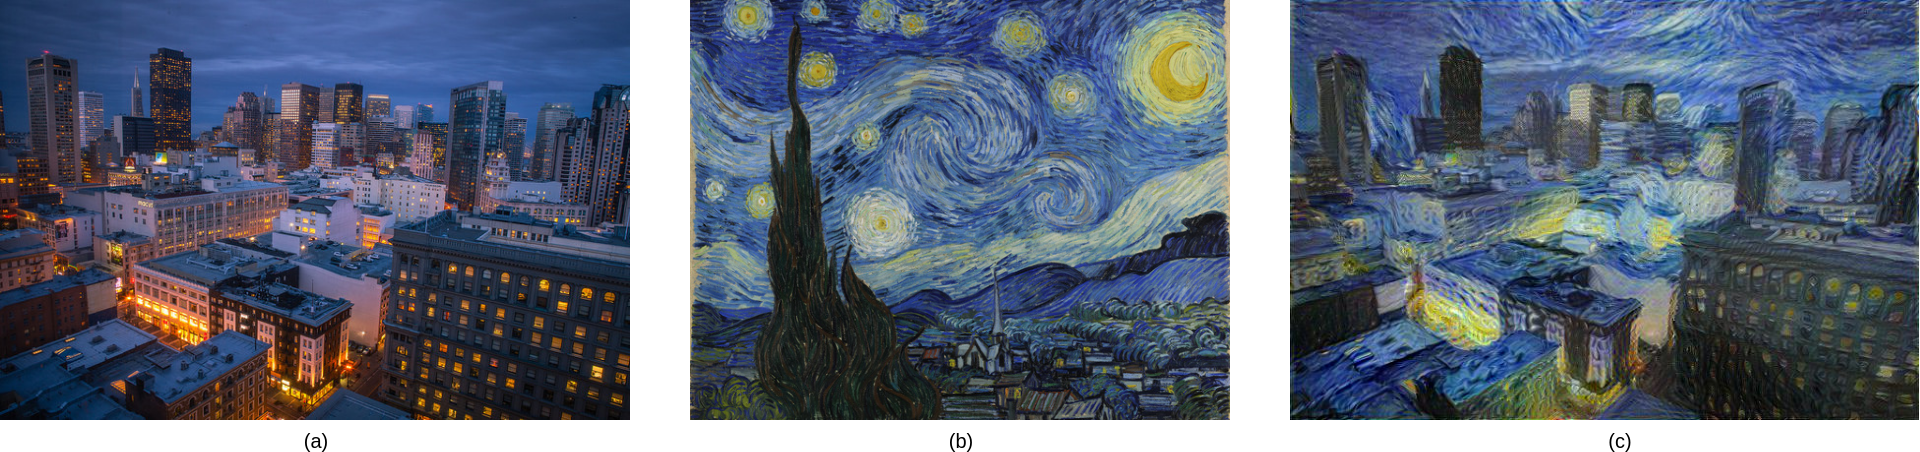
\includegraphics[width=\textwidth]{images/style-transfer-vision.png}
    \imgsrc{\url{https://github.com/fzliu/style-transfer}}
	\caption{\label{fig:style-transfer-vision}Sample of vision style transfer. Image (a) provides the content, image (b) provides the style and image (c) is the final generated image}
\end{figure}


\begin{table}[ht]
	\centering
	\begin{tabular}{ | p{.45\linewidth} | p{.45\linewidth} | }
		\hline
		\textbf{Input}                                              & \textbf{Output}                                      \\
		\hline \hline
		i will bite thee by the ear for that jest .                 & i ’ ll bite you by the ear for that joke .           \\
		\hline
		what further woe conspires against mine age ?               & what ’ s true despair conspires against my old age ? \\
		\hline
		how doth my lady ?                                          & how is my lady ?                                     \\
		\hline
		hast thou slain tybalt ?                                    & have you killed tybalt ?                             \\
		\hline
		an i might live to see thee married once , i have my wish . & if i could live to see you married, i ’ ve my wish . \\
		\hline
		benvolio , who began this bloody fray ?                     & benvolio , who started this bloody fight itself ?    \\
		\hline
		what is your will ?                                         & what do you want ?                                   \\
		\hline
		call her forth to me .                                      & bring her out to me .                                \\
		\hline
	\end{tabular}
	\imgsrc{\cite{xu2012paraphrasing}}
	\caption{Results of transferring authorship style from Shakespearean plays to modern english}
	\label{tab:paraphrasing-for-style-results}
\end{table}

This problem in the context of text was first introduced in by \cite{xu2012paraphrasing} as a statistical model that attempted to paraphrase bodies of text in a different style using a simple replacement strategy. An few examples from this paper are shown in Table \ref{tab:paraphrasing-for-style-results}. Since the overwhelming adoption of neural network based models in the NLP community, there have been several new bodies of work that break new ground in this area.


\section{Problem Statement}

The objective of this thesis is to perform an exploratory analysis of previous methods and test novel hypotheses that tackle the problem of the disentanglement of latent spaces of artificial neural networks and its applications to linguistic style transfer.

We operate under the following constraints and assumptions in our formulation of the problem:

\begin{itemize}
	\item The model is singular, with no conditional execution branch based on desired attribute. i.e. there is only one decoder and the number of decoders does not scale with the number of distinct transferrable attributes.
	\item The corpus of styles are non-parallel i.e. for instance, there are no pre-defined pairs of $(document_1, document_2)$ for style labels $\in (1, 2)$, as would be commonly seen in neural machine translation corpora.
	\item The corpora is annotated with the current attribute each document possesses e.g. each document has a corresponding `positive'/`negative' label if the task is to perform sentiment transfer.
	\item Optionally, a lexicon of words that are statistically very likely to be associated with each distinct class label would be useful, primarily to evaluate how well content has been preserved without penalizing change in vocabulary caused by the transferring of style.
\end{itemize}

The next chapter will delve deeper into the background required for an understanding of the models we implement and evaluate.


%======================================================================
\chapter{Background}
%======================================================================

\section{Natural Language Generation}

Natural Language Generation (NLG) is a sub-field of Natural Language Processing that attempts to generate sequences of words that resemble natural human languages. Traditionally, this was done either by using production rules of a pre-defined grammar, or by performing statistical analyses of existing human-written texts to predict sequences of words based on their occurrence probabilities. Markov-chain text generators are an example of the latter, popularized by their usage in parody text generation \cite{jelinek1985markov}.

This broad classification of problems has multiple applications include, and are not limited to:
\begin{itemize}
	\item Neural machine translation (NMT), in which the generation objective is to produce a semantically similar sentence in a target language, given a sentences in a source language.
	\item Dialogue generation, in which the objective is to produce a natural and syntactically correct response to the provided utterance.
	\item Text summarizaton, which eliminates superfluous and non-pertinent information in a body of text, to express the idea using fewer words.
	\item Data-to-text report generation, which utilizes structured data, sourced from a relational database format to fill out a text template.
\end{itemize}

\section{Recurrent Neural Networks}

Recurrent neural networks (RNNs) are a sub-class of artificial neural networks that can be considered a neural network equivalent to a Hidden Markov Model. Its units forms a directed graph that operates on a sequence of inputs when unrolled temporally. This makes them a useful tool for extracting features from arbitrary length sequences of input like audio or text. The features extracted at a given temporal point in an instance (sequence) is given by the below equation.
\begin{equation}
	P(w_1, \cdots, w_T) = \prod_{i=1}^T P(w_i | w_1, \cdots, w_{i−1})
\end{equation}

The language model is built in such a way that the features extracted from the sequence at epoch $t$ depend on the features observed during the epochs $0 \cdots t-1$. A graphical depiction of an unrolled RNN is shown in figure \ref{fig:recurrent-neural-network-unfold}.

\begin{figure}[ht]
	\centering
	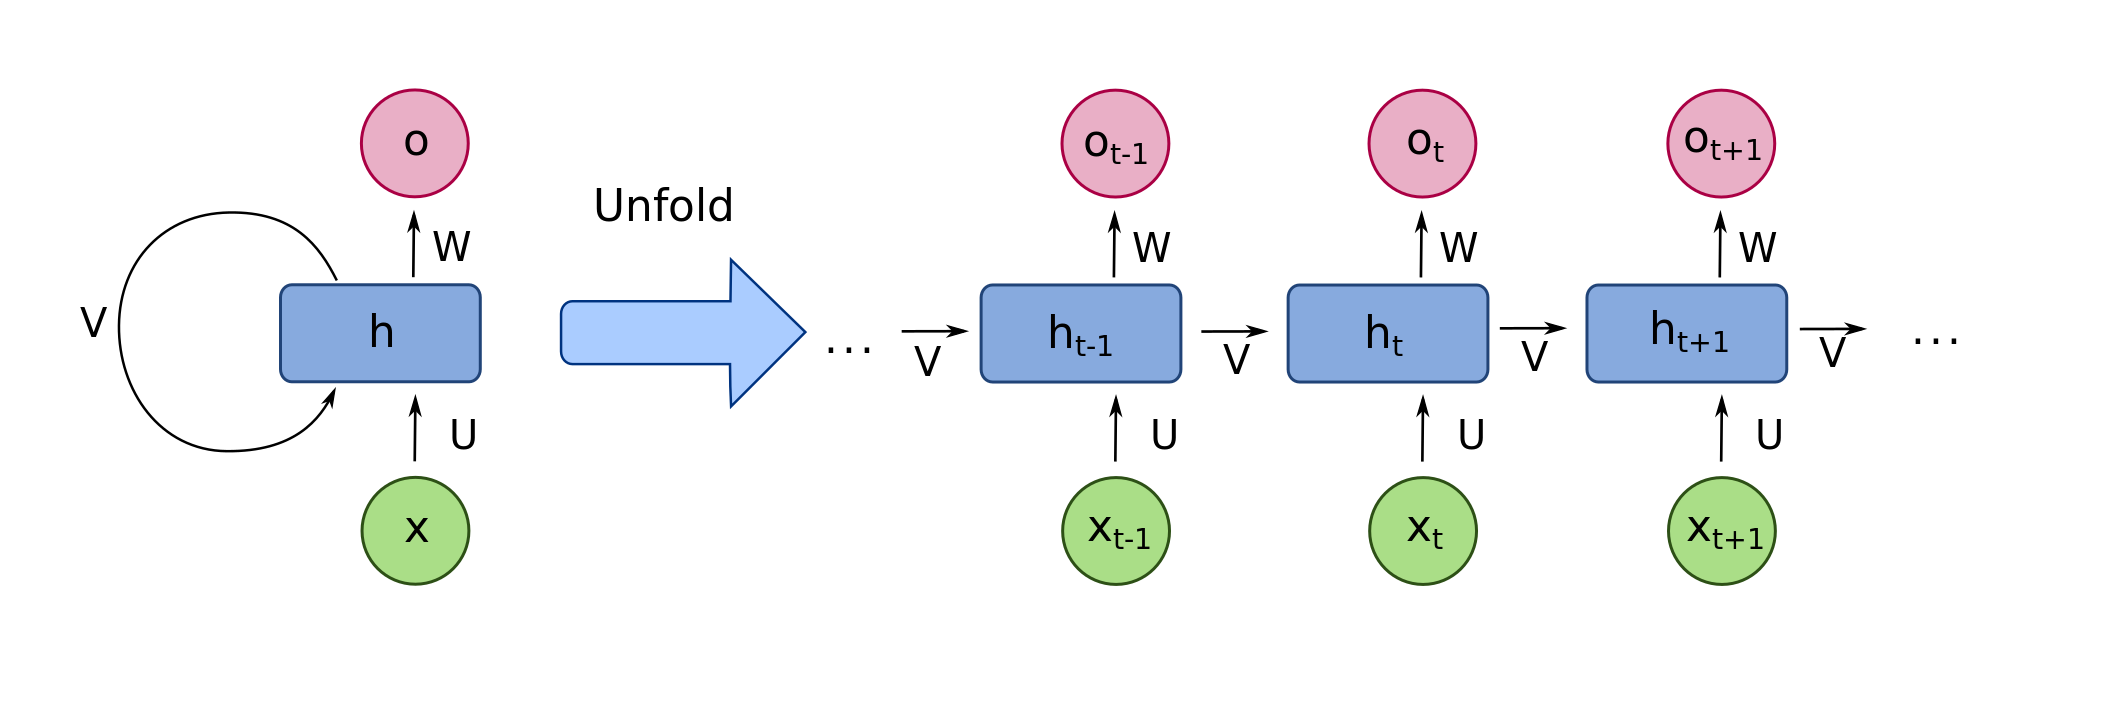
\includegraphics[width=\textwidth]{images/recurrent-neural-network-unfold}
	\imgsrc{\url{https://commons.wikimedia.org/wiki/File:Recurrent_neural_network_unfold.svg}}
	\caption{\label{fig:recurrent-neural-network-unfold} Unrolled RNN}
\end{figure}

The most recent and useful variants of recurrent units provide the ability to retain `memory' of the context in which the current features are to be considered. In the domain of language processing, this typically implies that the recurrent unit has a stored memory of the previously observed words in a sequence, and this property grants it the ability to learn context as part of the feature space.

The prominent variants of recurrent units used in neural networks to extract features from sequences using a memory mechanism, are Long Short-Term Memory (LSTM) units \citep{gers2001lstm} and Gated Recurrent units (GRU) \citep{chung2014empirical}.

Recurrent networks in the domain of natural language processing is used frequently for both natural language understanding (NLU) tasks, as well natural language generation (NLG) tasks. Similar to the manner in which recurrent networks can extract features from arbitrarily long sequences of vectorized text, they can also be used to produce text sequences from a unit vector representation of text, as represented in Figure \ref{fig:rnn-nmt}.

This is achieved by conditioning the generation of the first word of text either on some latent variable produced by a model, or by sampling from a generative distribution, and conditioning the generation of each subsequently predicted word on the word that was predicted in the previous time-step, until the model predicts an end-of-sentence (EOS) token.

\begin{figure}[ht]
	\centering
	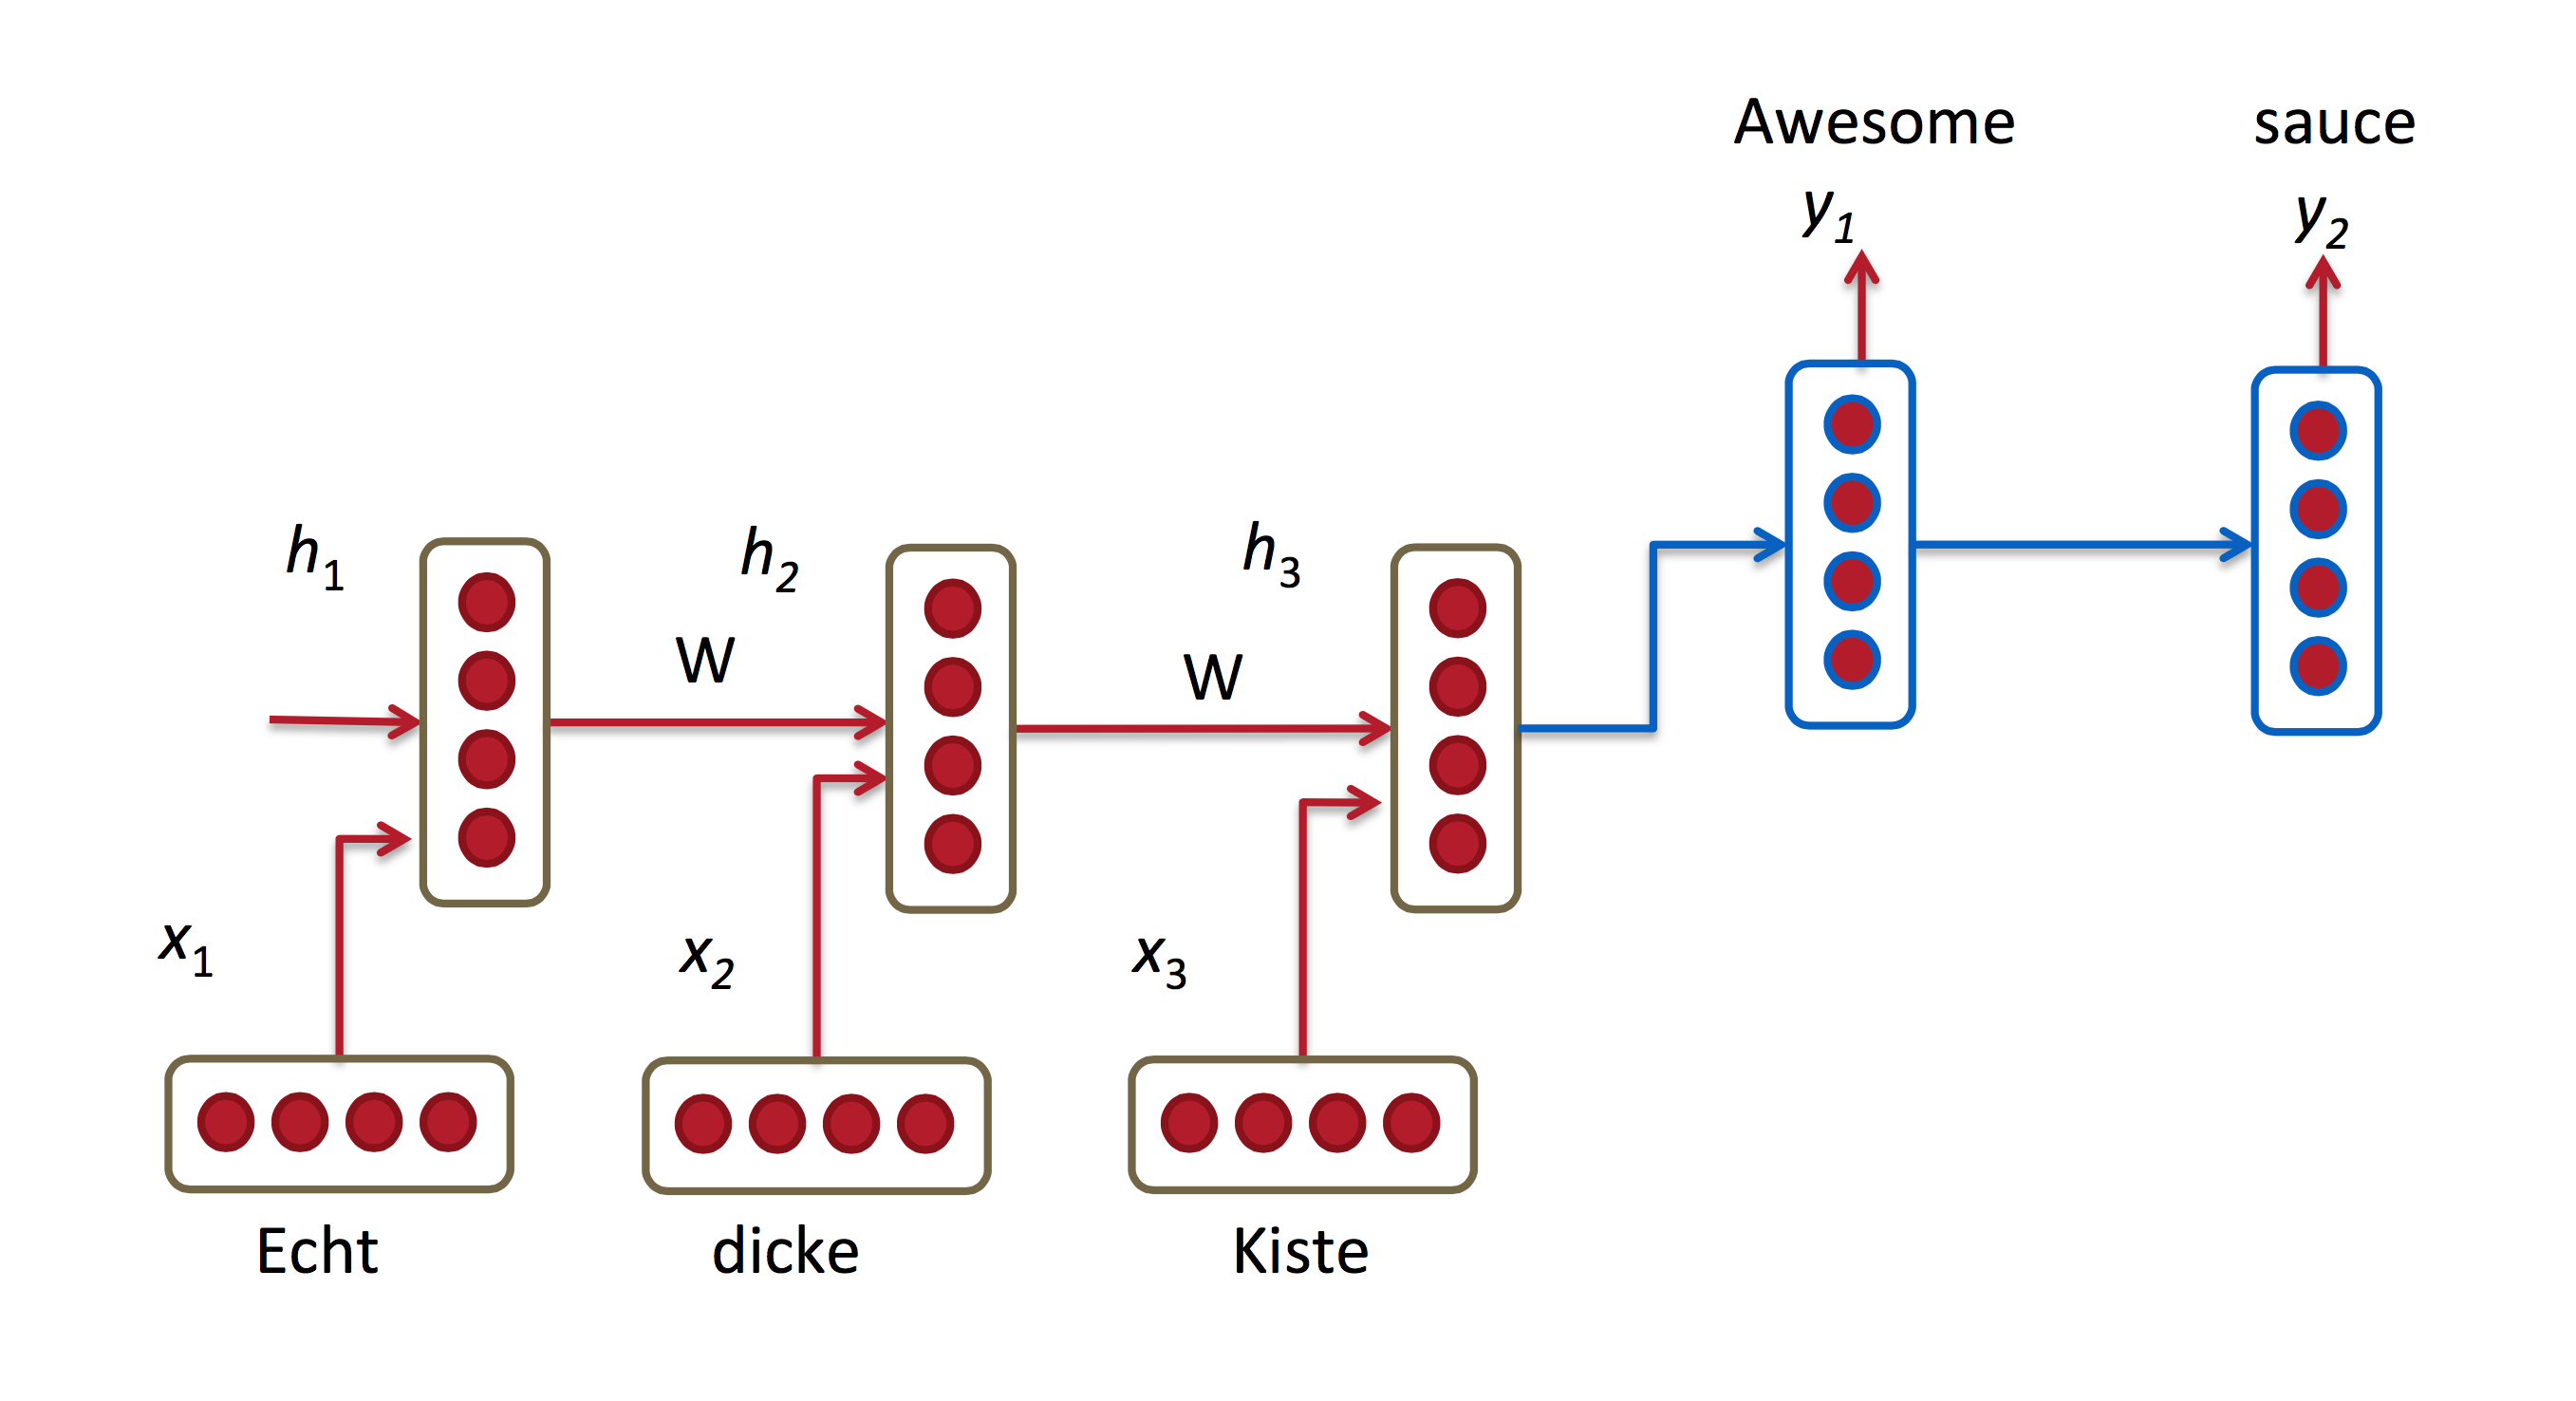
\includegraphics[width=\textwidth]{images/rnn-nmt}
	\imgsrc{\url{http://www.wildml.com/2015/09/recurrent-neural-networks-tutorial-part-1-introduction-to-rnns}}
	\caption{\label{fig:rnn-nmt} Recurrent Network Encoder-Decoder}
\end{figure}

\section{Autoencoders}

Autoencoders are models that are parameterized to convert arbitrary data into a latent representation (encoder), and recover the original data back from the latent representation (decoder). In this setup, the degrees of freedom for the latent representation is usually much smaller than that of the actual data. A simple autoencoder architecture is depicted in Figure \ref{fig:autoencoder-structure}.

\begin{figure}[ht]
	\centering
	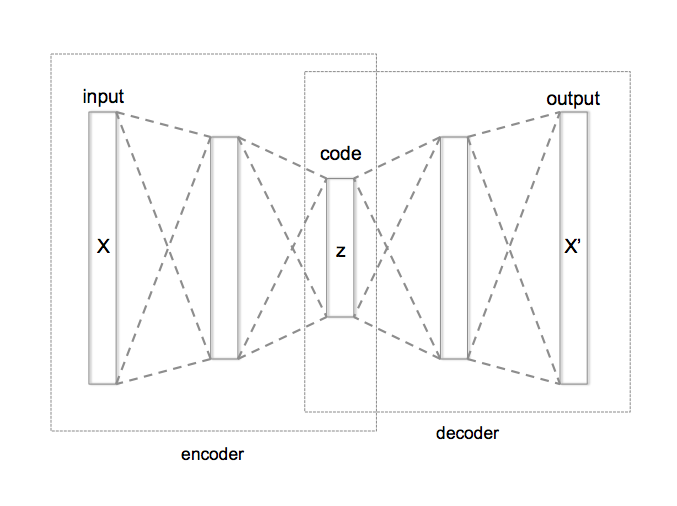
\includegraphics[width=\textwidth]{images/autoencoder-structure}
	\imgsrc{\url{http://mlexplained.com/2017/12/28/an-intuitive-explanation-of-variational-autoencoders-vaes-part-1}}
	\caption{\label{fig:autoencoder-structure} Autoencoder Architecture}
\end{figure}

By training a model to do this, two objectives can be achieved simultaneously:
\begin{itemize}
	\item The encoder weights of the model could be used extract the most salient features of the data in a compressed representation, which is a friendlier format for downstream processing or learning algorithms. \citep{hinton2006reducing}
	\item The decoder weights of the model could be used as a generator. Given that we can sample from the distribution of the existing latent representations learnt, or from a pre-defined prior (in a variational autoencoder), we can generate plausible novel data.
\end{itemize}

In the context of natural language the encoder can be utilized as a sentence-encoding feature-extractor and the decoder can be utilized as a generative model. Autoencoders are also used for being able to de-noise data given pairs of noisy and regular data, by learning a de-noising function. These properties make autoencoders a good framework to utilize to implement sequence-to-sequence models, where both the encoder and decoder weights of the network are parameterized by recurrent neural networks.

\subsection{Variational Autoencoders}

Variational encoders (VAEs) \citep{kingma2013auto} are a probabilistic variant of autoencoders. The general structure of a VAE is the same as that of a deterministic autoencoder, with an encoder that learns a compressed latent space and a decoder that learns a function to map the latent space into the original data. A simple VAE architecture is depicted in Figure \ref{fig:vae-structure}.

\begin{figure}[ht]
	\centering
	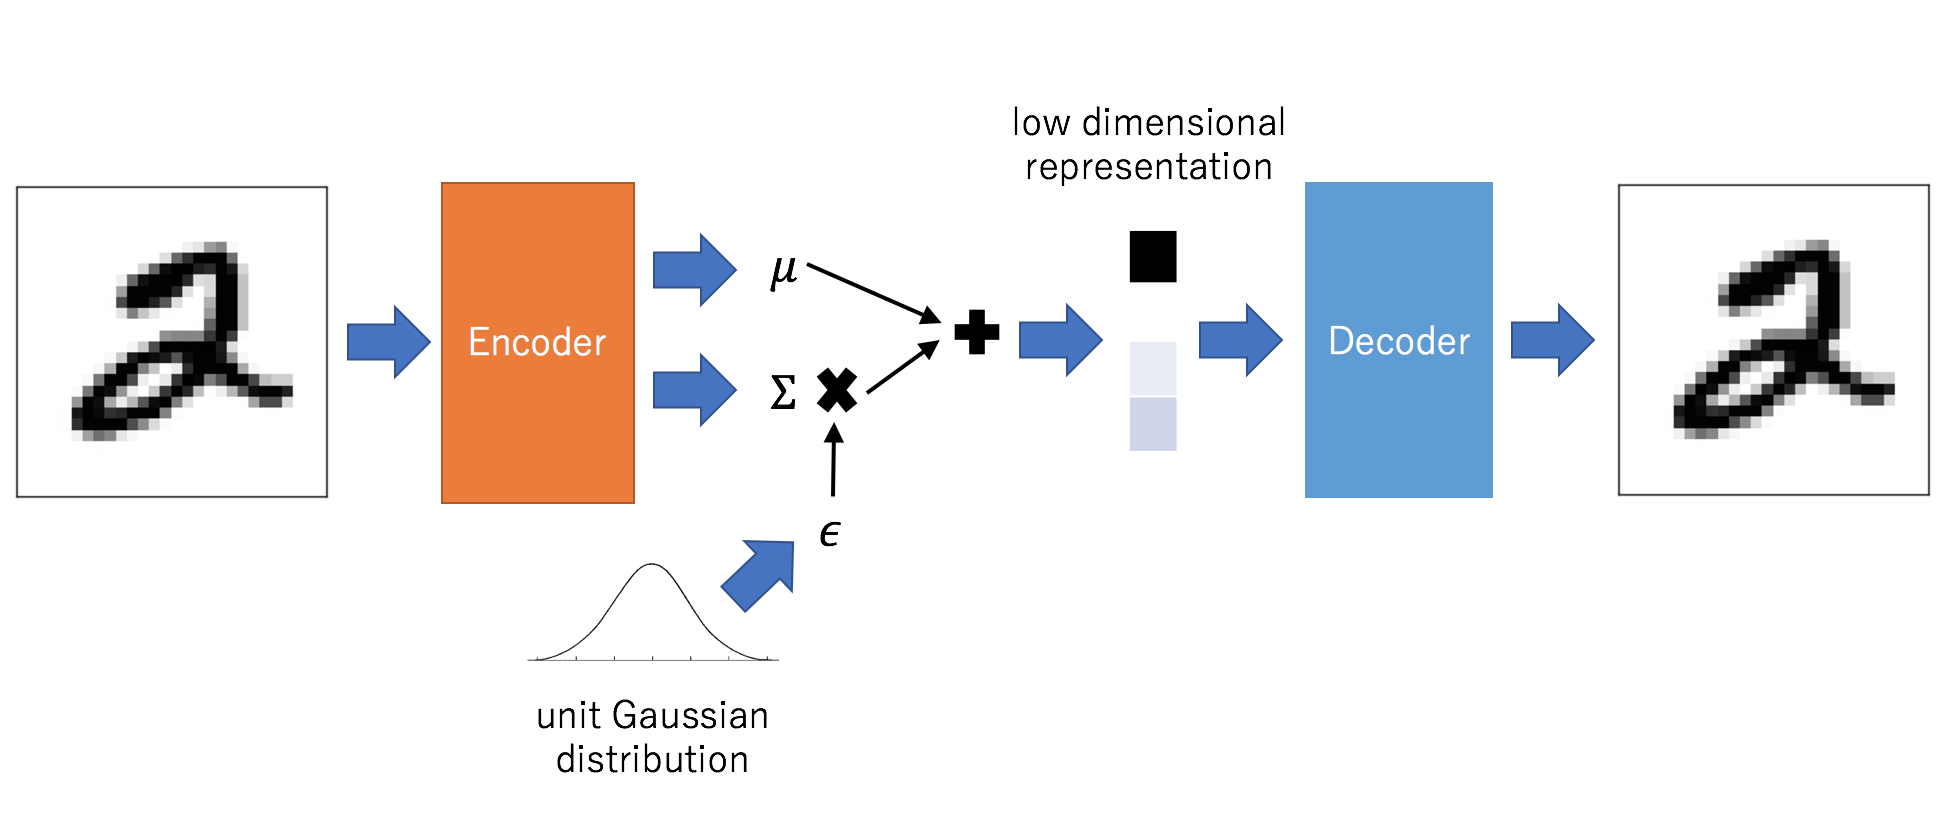
\includegraphics[width=\textwidth]{images/vae-structure}
	\imgsrc{\url{http://mlexplained.com/2017/12/28/an-intuitive-explanation-of-variational-autoencoders-vaes-part-1}}
	\caption{\label{fig:vae-structure} VAE Architecture}
\end{figure}

In contrast to the deterministic autoencoder we observe that a variational inference networks autoencoder learns representations of both the mean and variance latent spaces. The method requires placing conjugate priors on the mean and variance of the unknown latent representation. The encoder then tries to learn the approximate posterior distribution. This family of distributions used for this purpose are Gaussian.

In addition to the reconstruction loss that a deterministic autoencoder uses, a metric of distance is used to evaluate how closely between the learned representations of mean and variance resemble a Gaussian distribution with mean 0 and unit variance. The Kullback-Leibler (KL) divergence \citep{kullback1951information} is used to penalize learned representations that do not resemble the prior. However, we cannot compute the KL directly. Instead we compute an alternative objective that is equivalent to the KL upto an added constant. This is called the evidence lower-bound (ELBO). The ELBO objective maximized in a variational autoencoder model is given below:

\begin{equation}
	ELBO(q) = \mathbb{E}_{q(z)} [(\log(p(x|z))] - \mathbb{KL}(q(z)||p(z))
\end{equation}

Simultaneously, for the decoding step, we sample from the prior, utilizing the re-parameterization trick to ensure that the model remains differentiable. As a result the decoder is trained as a generative network that can randomly sample from the prior and generate plausible data similar to the input distribution. The decoder being able to act as a generative model independently is what sets a VAE apart from a generative model.

\section{Sequence to Sequence Modeling}

Also abbreviated in the literature as Seq2Seq, this is a class of models that learns functions that map from one sequence to another. First introduced by \cite{sutskever2014sequence}, the general premise of sequence to sequence has been a flexible framework for modelling transformations made to arbitrary length sequences. In the natural language processing community, the main tasks that benefit from the encoder-decoder framework are neural machine translation, dialogue modeling, question answering for which there exists two distinct distributions of data, and the model is trained to learn the mapping from one to the other.

The paper defines a sequence-to-sequence model as on that learns the below function to map a sequence of inputs $x_1, ... , x_T$ to a sequence of outputs $y_1, ... , y_{T′}$, where the initial state $h$ is set to the hidden LSTM representation of $x_1, ... , x_T$.

\begin{equation}
	p(y_1, ... , y_{T′} | x_1, ... , x_T) =	\prod_{t=1}^T p(y_t | h, y_1, ... , y_{t−1})
\end{equation}

This makes the Seq2Seq model an ideal framework using which one can implement solutions to several natural language generation tasks like neural machine translation, dialogue generation, text summarizaton etc.

\section{Adversarial Networks}

\cite{goodfellow2014generative} present a new model that utilizes the idea of a game-theoretic competition between the generative model which is a decoder, and a discriminative model which is usually a classifier or regressor. The general idea is to train the adversary to be able to discriminate between the distributions that the generator model is trying to produce and a true distribution, that it the generator trying to mimic.

\begin{figure}[ht]
	\centering
	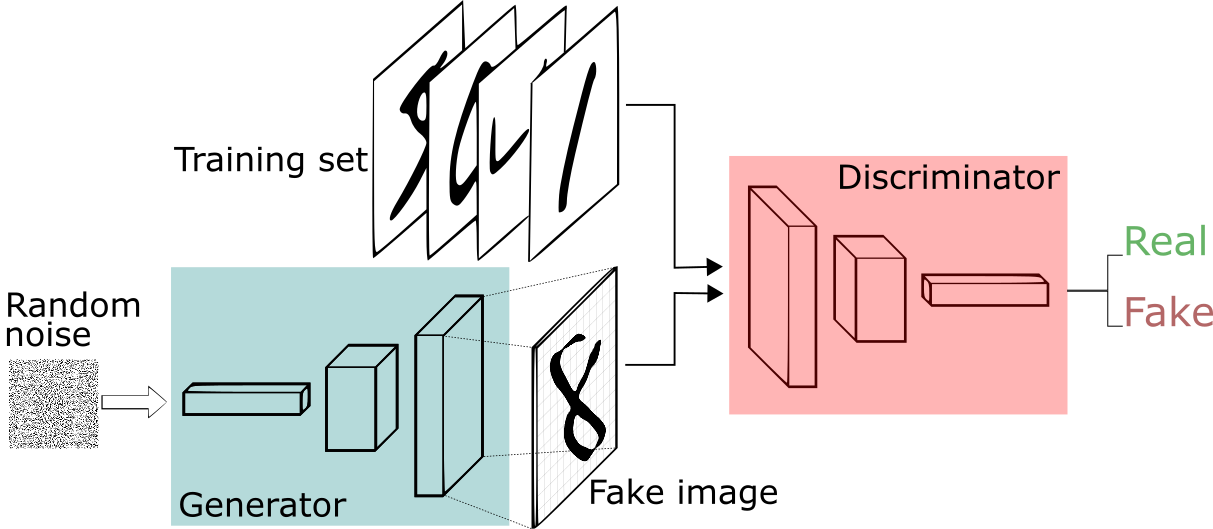
\includegraphics[width=\textwidth]{images/gans}
	\imgsrc{\url{https://deeplearning4j.org/generative-adversarial-network}}
	\caption{\label{fig:gans} GAN Architecture}
\end{figure}

In the original formulation of adversarial training, which involves using a binary classifier, the generator learns weights to map a randomly initialized latent variable $z$ to a data distribution $x$ that it is unaware of. The discriminator is trained using the true distribution and samples generated by the generative model, and it's objective is to discriminate the true samples from the generated samples. The generator on the other hand, attempts to maximize the discriminator's classification error, thereby producing plausible samples that mimic the true distribution.

This property of the generator model parameters possess, of translating random noise into plausible data samples are used in areas of research within computer vision and natural language processing to produce novel data. Also adversarial learning as a principle is a great tool to ensure that known partial information present in the latent space is disentangled from any arbitrarily chosen sub-space.

We utilize adversarial learning in our model to assist with the disentanglement of style labels.


\section{Image Style Transfer}

The idea of neural style transfer in the was originally proposed by \cite{gatys2016image}. In the task described in the paper, the authors use two distinct images as input. The first image contributes the content, and the second contributes the style. The objective is to generate a final image that contains all of the physical objects visible in the first image, but depicted by the style (hue, brush strokes, texture etc.) visible in the second.

\begin{figure}[ht]
	\centering
	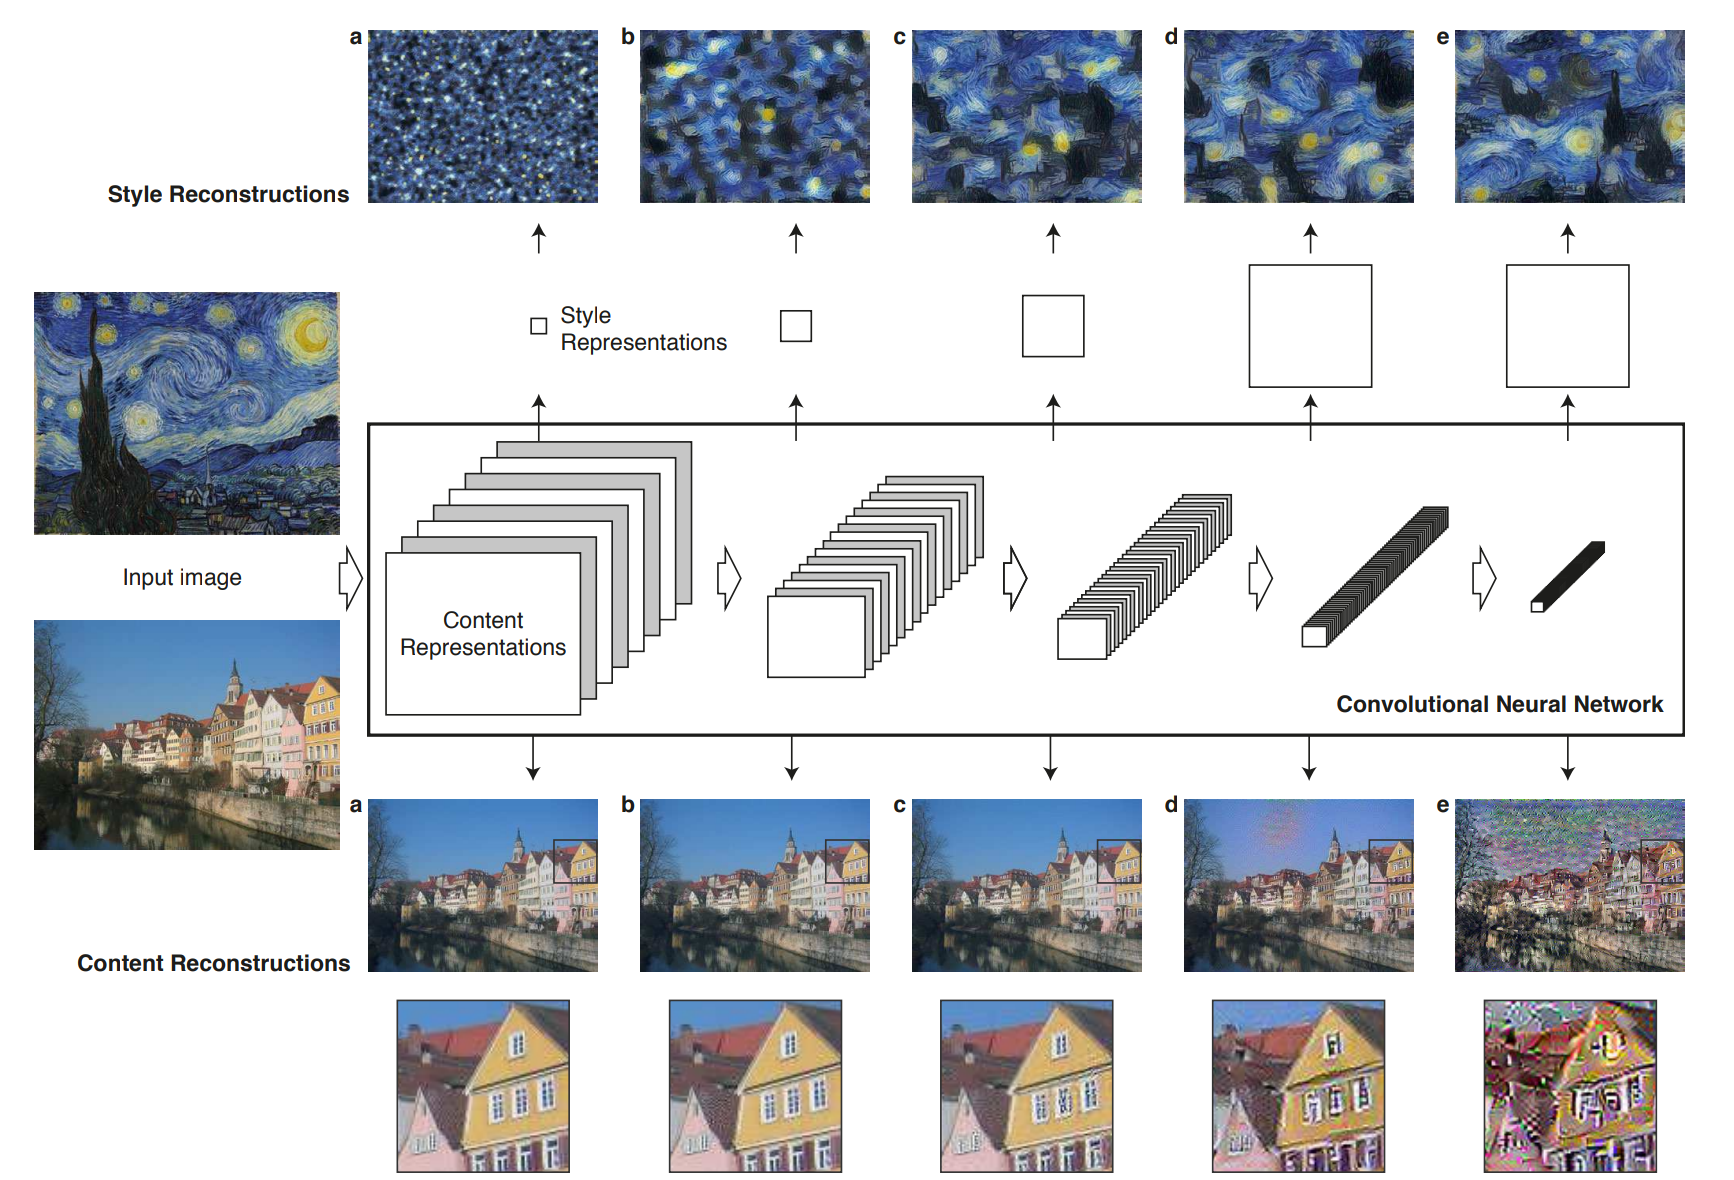
\includegraphics[width=\textwidth]{images/image-style-transfer.png}
	\imgsrc{\cite{gatys2016image}}
	\caption{\label{fig:image-style-transfer} Artistic Style Transfer in Images}
\end{figure}

The features, as with most of the state-of-the-art image processing techniques, are extracted from the images using Convolutional Neural Networks (CNNs) \citep{lecun1998gradient}, the deep neural network variants of which have been widely successful at image recognition tasks such as object recognition in the ImageNet data-set \cite{krizhevsky2012imagenet}.

As depicted in Figure \ref{fig:image-style-transfer}, subsequent layers of the CNN learn incrementally higher level features in both the style image and the content image. These learned features for the style and content images are stored for uture use. To generate the final image, the authors begin with a random white noise image. This image is passed through both networks, the parameters of which extract both it's style features and it's content features.

This model uses two training objectives:
\begin{itemize}
	\item Minimize the the element-wise mean squared difference between the style features computed for the style image and the white-noise image
	\item Minimize the the mean squared difference between the content features of the content image and the white noise image, as shown in the below equations.
\end{itemize}

The overall training loss is a linear combination of the above objectives, and is used to iteratively modify the white-noise image until it the style features of the style image and the content features of the content image.

The next chapter builds on the fundamentals established in this one, and discusses previous attempts at neural disentanglement in the context of linguistic style transfer as well as methods that do not use disentanglement as the basis of the style transfer model.


%======================================================================
\chapter{Related Work}
%======================================================================

In the past year, the work by \cite{hu2017toward} and \cite{ficler2017controlling} both expounded the applicability of attribute-conditioned generated to linguistic style transfer tasks. Both of these methods, as opposed to the historical used paraphrasing methods \citep{xu2012paraphrasing}, utilized neural network models \citep{lecun2015deep} to learn the style transfer function.

Further work presented by \cite{shen2017style} and \cite{fu2017style} utilize the idea of removing attribute information from latent representations using adversarial learning. In this section we discuss some of the prominent work done in this area.

\section{Controlled Generation of Text}

\cite{hu2017toward} use a variational autoencoder trained with the reconstruction objective and a KL-divergence minimization objective on the latent space with respect to a prior $p(z)$, as described in the original variational auto-encoding paper by \cite{kingma2013auto}. In addition to the reconstruction objective, the authors use additional discriminative training signals to adapt the desired attributes of the generated text. These training signals need to be propagated back to the encoder.

$x$ is the source corpus and the encoder is parameterized to generate a latent code $z$, which is a variational latent space that resembles a Gaussian prior. (This is enforced by a KL-divergence loss). The structured code $c$ is a known label of the text (discrete or continuous). The decoder generator produces the output corpus $\hat{x}$ conditioned on $(z, c)$. It uses greedy decoding, which predicts the word with maximal probability at each step \citep{langlais2007greedy}.

A classifier/regressor discriminator predicts the structured code of the output corpus $\hat{x}$ to ensure that it is the same as the one the generator was conditioned on i.e. $G(z, c)$. The discriminator is pre-trained.

Each decoder step in $\hat{x}$ is predicted using a softmax function scaled by a temperature $\tau$. Higher temperatures flatten the softmax distribution for each word prediction and increase word diversity. Conversely, setting $\tau = 0$ will resemble a discrete probability distribution over the corpus vocabulary. For their experiments, the authors gradually anneal $\tau \rightarrow 0$

The authors describe the following objectives to train their model:

\subsection{Variational Autoencoder}

A reconstruction loss that ensures that the generated sentence $\hat{x}$ is the same as the original sentence $x$. This is equivalent to minimizing the negative log-likelihood of generating $\hat{x}$. This is shown in Equation \ref{eqn:tcg-rec}
\begin{eqnarray} \label{eqn:tcg-rec}
	\mathcal{L}_{VAE}(\theta_G, \theta_E; x) &=& \nonumber
	- \mathbb{E}_{q_E(z|x)q_D(c|x)}[log p_G(x|z,c)] \\ & &
	+ KL(q_E(z|x)||p(z))
\end{eqnarray}


\subsection{Style Discriminator}

A discriminator validates if the predicted class/value for $\hat{x}$ is the same as the corresponding class/label for $x$. This is a cross-entropy loss over the probability distribution of the labels. This discriminator loss can be further subdivided into 2 terms, one that maximizes the log likelihood of predicting the correct class as in Equation \ref{eqn:tcg-disc-class}, and one that minimizes the empirically observed Shannon entropy of the predicted distribution, thereby incentivizing confident predictions, as in Equation \ref{eqn:tcg-disc-ent}.
\begin{equation} \label{eqn:tcg-disc-class}
	\mathcal{L}_s(\theta_D) = - \mathbb{E}_{X_L}[log q_D(c_L|x_L)]
\end{equation}
\begin{equation} \label{eqn:tcg-disc-ent}
	\mathcal{L}_u(\theta_D) = - \mathbb{E}_{p_G(\hat{x}|z,c)p(z)p(c)}
	[log q_D(c|\hat{x}) + \beta \mathcal{H}(q_D(c'|\hat{x}))]
\end{equation}


\subsection{Content Discriminator}

The encoder from loss equation \ref{eqn:tcg-rec}, is used to regenerate the latent distribution $z$ devoid of the structured code from the output distribution $\hat{x}$. The authors call this an \textbf{independence constraint}, in that regardless of the structured code $c$ that is currently present in either $x$ or $\hat{x}$, processing either through the generator should produce a consistent $z$. This allows the encoder to encode only latent factors that are independent of the structured code. This is shown in Equation \ref{eqn:tcg-ind-con}.
\begin{equation} \label{eqn:tcg-ind-con}
	\mathcal{L}_{attr, z}(\theta_G) = - \mathbb{E}_{p(z)p(c)}
	[log q_E(z|\tilde{G_{\tau}}(z,c))]
\end{equation}


They maximize the expected log likelihood of predicting the correct distribution of the structured code $c$ given the labelled examples $X_L$. This happens before the generator model training. They also maximize the expected log likelihood of predicting the correct distribution of the structured code $c$ given the generated sentences $\hat{x}$. Also minimize the empirically observed Shannon entropy of the observed discriminator prediction $q_D(c'|\hat{x})$, which reduces uncertainty and increases confidence of the structured code prediction. A wake-sleep algorithm \citep{hinton1995wake} is used to alternatively train the generator and discriminator.

The model was applied only to short sentences with length $<15$ words and the encoder-decoder setup is implemented using single layer LSTMs and the discriminator is implemented using a convolutional neural network (CNN). The KL loss weight is annealed from 0 to 1 during training.


\section{Aligned and Cross-Aligned Autoencoders}

\cite{shen2017style} aim to perform style transfer on language using non-parallel corpora by separating content from style. They re-align the latent spaces to perform three tasks: sentiment modification, decipherment of word-substitution ciphers, and recovery of word order. Their method involves learning an encoder that takes a sentence and its original style label as input, and maps it to a content representation devoid of style. This representation is then decoded by a decoder whose input is this encoded representation and the target style label.

There are two non-parallel corpora $X_1 = {x_1^{(1)} ... x_1^{(n)}}$, drawn from the prior $p(x_1|y_1)$ and $X_2 = {x_2^{(1)} ... x_2^{(n)}}$, drawn from the prior $p(x_2|y_2)$. The objective is to estimate the style transferred distributions $p(x_1|x_2;y_1,y2)$ and $p(x_2|x_1;y_1,y2)$.

The authors propose a constraint that $x_1$ and $x_2$'s marginal distributions can only be recovered if for any different styles $y, y' \in Y$, distributions $p(x|y)$ and $p(x|y')$ are different, which is a fair assumption to make because if $p(x|y)$ = $p(x|y')$, then the style changes would be indiscernible.

They also prove that if the content $z$ is sampled from a centered isotropic distribution, the styles cannot be recovered from $x$, but in the case of $z$ being a more complex distribution like a Gaussian mixture, then the affine transformation that converts $y, z$ into $x$ can be recovered.

The reconstruction loss is the same as the one used by a variation autoencoder for its reconstruction objective, as shown in Equation \ref{eqn:stca-rec}.
\begin{eqnarray} \label{eqn:stca-rec}
	\mathcal{L}(\theta_E,\theta_G)
	&=& \mathbb{E}_{x_1 \sim X_1}[-\log p_G(x_1|y_1,E(x_1, y_1))] \nonumber \\
	& & + \mathbb{E}_{x_2 \sim X_2}[-\log p_G(x_2|y_2,E(x_2, y_2))]
\end{eqnarray}

\subsection{Aligned Autoencoder}

The authors propose aligning the distributions $P_E(z|x_1)$ and $P_E(z|x_2)$ where $E$ is the encoder function. This is done by training an adversarial discriminator to distinguish between the two distributions.

The adversarial objective is expressed as below where $D(\cdot)$ predicts 0 if it predicts the source distribution to be $X_1$ and 1 if it predicts the source distribution to be $X_2$
\begin{eqnarray} \label{eqn:stca-align-adv}
	\mathcal{L}_{adv}(\theta_E,\theta_D)
	&=& \mathbb{E}_{x_1 \sim X_1}[-\log D(E(x_1,y_1))] \nonumber \\
	& & + \mathbb{E}_{x_2 \sim X_2}[-\log(1 - D(E(x_2,y_2)))]
\end{eqnarray}

The overall optimization objective combining equations \ref{eqn:stca-rec} and \ref{eqn:stca-align-adv} can be written as
\begin{equation}
	\mathcal{L} = \operatorname*{min}_{E,G} \operatorname*{max}_{D} \mathcal{L} - \lambda \mathcal{L}_{adv}
\end{equation}
where $\lambda$ is a balancing weight for the adversarial term.

\subsection{Cross-aligned Autoencoder}

This is similar to the aligned autoencoder approach, but instead of trying to align $P_E(z|x_1)$ and $P_E(z|x_2)$ using an adversarial discriminator, two distinct adversarial discriminators are used to align a sequence of real and transferred generator hidden states. i.e. $D_1$ is used to align the distributions $G(y_1, z_1)$ and $G(y_1, z_2)$. Similarly, $D_2$ is used to align the distributions $G(y_2, z_2)$ and $G(y_2, z_1)$. These discriminators are trained with the objective of being unable to identify the content distributions $P(z_1)$ and $P(z_2)$

Professor-forcing is used to train both of these discriminators. Professor forcing uses a discriminator to distinguish if the decoder hidden states are a result of training-time teacher forcing or test time scheduled sampling \citep{lamb2016professor}. This is a generalized version of simply using a final encoder state, as was the case in the Aligned Autoencoder solution.

The overall optimization objective combining equation \ref{eqn:stca-rec} and two discriminator variants of equation \ref{eqn:stca-align-adv} can be written as:
\begin{equation}
	\mathcal{L} = \operatorname*{min}_{E,G} \operatorname*{max}_{D} \mathcal{L} - \lambda (\mathcal{L}_{adv_1} + \mathcal{L}_{adv_2})
\end{equation}

As opposed to the simple feed-forward classifier used in the aligned autoencoder, the cross-aligned autoencoder uses convolutional nets for text classification. They use Yelp reviews as the data set with rating $>3$ as positive and rating $<3$ as negative examples. Reviews with a sentence count $>10$ and sentences with a word count $>10$ are filtered out. The vocabulary size used is $10K$. Style transfer is evaluated using a pre-trained classifier. Language fluency and content preservation was evaluated using human assessments.

\section{Style Embedding Autoencoder}

\cite{fu2017style} employ two distinct models to perform style transfer
\begin{itemize}
	\item A \textbf{multi-decoder model} that use the distinct decoders to produce text in different styles. This implicitly means that the number of decoders that need to be trained scales with the number of distinct label values to train.
	\item A \textbf{style-embedding model} with a single decoder that generate text in different styles. This method utilizes a separate style embedding matrix, of size $n * m$ where $n$ is the number of distinct label values and $m$ is an arbitrarily chosen embedding size.
\end{itemize}

In contrast with the previous models described, this work uses a deterministic autoencoder in lieu of a variational autoencoder. For our purposes, we focus on the style-embedding model, since it requires explicit disentanglement and uses fewer model parameters for each label addition, compared to the multi-decoder model.

The training objectives used for this model include the reconstruction objective for the autoencoder, the style label discriminative objective for a classifier on the latent space, and the adversarial loss propagated back to the autoencoder from the representation learned in the content space.

The autoencoder is trained to product only the salient features that represent the content of the sentences i.e. the content space, and the style embedding vector is trained via back-propagation of the reconstruction loss.

The reconstruction loss is the same as that of a standard deterministic autoencoder.
\begin{equation}
	\mathcal{L}_{seq2seq} = -\sum_{i=1}^M \log P(\hat{x}_i|x_i;\theta_e;\theta_d)
\end{equation}
where $M$ is the number of training examples and $\theta_e$ and $\theta_d$ are the encoder and decoder parameters respectively.

A discriminative classifier is trained on the latent content space learned by the autoencoder, to distinguish between the different possible styles.
\begin{equation}
	\mathcal{L}_{disc} = -\sum_{i=1}^M \log P(l_i|Encoder(x_i;\theta_e);\theta_c)
\end{equation}
where $M$ is the number of training examples and $\theta_e$ and $\theta_c$ are the encoder and discriminative classifier parameters respectively.

An adversarial objective is applied to the content representation. This objective aims to maximize entropy of the predicted label from the content representation by minimizing the following objective:
\begin{equation}
	\mathcal{L}_{adv} = -\sum_{i=1}^M\sum_{j=1}^N \mathcal{H}(P(j|Encoder(x_i; \theta_e); \theta_c))
\end{equation}
where $M$ is the size of the training data and $N$ is the number of distinct styles. Using this adversarial entropy objective, the encoder is penalized and therefore trained to produce a latent content representation which is independent of style.

Similar to the persona-based neural conversation model \citep{li2016persona}, a style embedding is learned for each different style. The conditional generation is done using recurrent neural networks with the inputs being the recurrent networks current state, and the style embedding to apply.

The style embeddings matrix is not directly parameterized by the encoder, but the learning algorithm propagates changes based on how well it combines with the content representation to reconstruct the original text.

The methods are evaluated in the following manner:
\begin{itemize}
	\item Transfer strength is evaluated using a simple classifier
	\item Content preservation is evaluated by computing the cosine distance between the original and the generated text embeddings.
\end{itemize}


Several other works have also been published in this domain recently including using cyclical translation to strip style as a pre-processing step, followed by a multi-decoder model to generate style-transferred sentences \citep{prabhumoye2018style},

\todo[inline]{Add related work in CV/NLP}


%======================================================================
\chapter{Challenges}
%======================================================================

\section{Non-interpretable Latent Representations}

The randomness and inscrutability of the learning processes in neural networks has prompted research into learning interpretable representations \citep{chen2016infogan}.

Although neural networks have proved to be highly capable function approximators in the general machine intelligence literature over the past couple of decades, without any explicit additional modeling, the weights of a neural network are learnt in an arbitrary manner to approximate a function modeled by a user-defined loss variable.

Due to this non-explainability of the weights of neural networks, they have been used as a black-box in practice, and the non-explainability hampers their adoption in use-cases required explicit audits and accountability, and for humans to reason about why a system chose a particular outcome over the other options available.

We believe that the disentanglement of the learned weights of a neural network are an important step in the direction of addressing this shortcoming, using available labels to force representation learning to adhere to a pre-defined separation scheme in the latent space.


\section{Quantitative Evaluation of Language Quality}

The evaluation of novel generated text to measure its perceived quality, naturalness, fluency and compliance with predefined attributes, like sentiment, tense etc.

For the presence of a certain attribute, it is fairly simple to devise a classification model that is trained on a large corpora of samples labeled as such.

However it is much more difficult to unambiguously state what makes a body of text more fluent or natural that another with mathematical rigor using quantitative metrics.

To offset this problem while stilling avoiding the need for human annotators to evaluate the target text, we have utilized techniques like sentences embedding similarity, augmented by the removal of words that highly correlate with any specific label, as proposed by the previous work by \cite{fu2017style}. This is described further in section \ref{ssec:content-preservation-metric} of the Experiments chapter.


%======================================================================
\chapter{Approach}
%======================================================================

This work provides a novel approach to solve this open problem, and juxtaposes this approach and its experimental results against the current state-of-the-art models. We empirically demonstrate the separation of content and style spaces by demonstrating the inferred spaces of labeled sentences in a sentiment-transfer task, where the positive sentences in the test set are converted to equivalent sentences with a negative sentiment, and vice-versa. We open-source our implementation under a permissive license so that the general framework can be applied to a multitude of other problems that are thematically similar, and rely on modifications of latent attributes in text.

In this section, we describe our approach in detail. Our model is built upon an autoencoder with a sequence-to-sequence (Seq2Seq) neural network~\cite{sutskever2014sequence}, as described in Subsection~\ref{ss:seq2seq}. Then we introduce two auxiliary losses, multi-task loss and adversarial loss in Subsections~\ref{ss:multi} and \ref{ss:adv}, respectively. Subsection~\ref{ss:prediction} presents the approach to transfer style in natural language generation. Figure~\ref{fig:model-overview} depicts both training and prediction processes of our approach.

\begin{figure}[ht]
	\centering
	\includegraphics[width=0.9\linewidth]{images/model-overview.png}
	\caption{Overview of our approach.}
	\label{fig:model-overview}
\end{figure}

\subsection{Autoencoder}\label{ss:seq2seq}

An autoencoder encodes an input to a latent vector space, from which it decodes the input itself. By doing so, the autoencoder learns meaningful representations of data. This serves as our primary learning objective. Besides, we also use the autoencoder for text generation in the style-transfer application.

Let $\rmx=(x_1, x_2, \cdots x_n)$ be an input sentence. The encoder encodes $\rm x$ by a recurrent neural network (RNN) with gated recurrent units (GRU) \cite{cho2014learning}, and obtains a hidden state $\bm h$.

Then a decoder RNN generates a sentence, which ideally should be $\rmx$ itself. Suppose at a time step $t$, the decoder RNN predicts the word $x_t$ with probability $p(x_t|\bm h, x_1\cdots x_{t-1})$, then the autoencoder is trained with cross-entropy loss, given by
\begin{equation}\nonumber
	J_\text{rec}(\bm\theta_E,\bm\theta_D)= -\sum_{t=1}^n \log
	p(x_t|\bm h, x_1\cdots x_{t-1})
\end{equation}
where $\bm\theta_E$ and $\bm\theta_D$ are the parameters of the encoder and decoder, respectively.

Since this loss trains the autoencoder to reconstruct $\rmx$, it is also called \textit{reconstruction loss}.

Besides the above reconstruction loss, we design two auxiliary losses to disentangle the latent space $\bm h$. In particular, we hope that $\bm h$ can be separated into two spaces $\bm s$ and $\bm c$, representing style and content respectively, i.e., $\bm h = [\bm s ; \bm c]$, where $[\cdot;\cdot]$ denotes concatenation. This is accomplished by the below auxiliary losses.

\subsection{Multi-Task Loss} \label{ss:multi}

Our first auxiliary loss ensures the style space does contain style information. We build a classifier on the style space $\bm s$ predicting the style label $s$, which is a part of the training data.

This loss can be viewed as a \textit{multi-task} loss, which makes the neural network not only decode the sentence, but also predicts its sentiment. Similar multi-task losses are used in previous work for sequence-to-sequence learning \cite{luong2015multi}, sentence representation learning \cite{jernite2017discourse} and sentiment analysis \cite{balikas2017multitask}, among others.

In our application, we follow previous work \cite{hu2017toward,shen2017style,fu2017style} and treat the sentiment as the style of interest. We introduce a binary classifier
\begin{equation}
	p(s=1|\bm s;\bm\theta_\text{mult})=\sigma(\bm w_\text{mult}^\top \bm s + b_\text{mult})
\end{equation}
where $\bm\theta_\text{mult}=[\bm w_\text{mult}; b_\text{mult}]$ are the classifier's parameters for multi-task learning.
\begin{align} \label{eqn:Jmult}
	 & J_\text{mult}(\bm\theta_{E};\bm\theta_\text{mult})=                \\ \nonumber
	 & -s\log p_\text{mult}(s|\bm s) - (1-s)\log p_\text{mult}(1-s|\bm s)
\end{align}
where $\bm\theta_E$ are the encoder's parameters. (Notice that the bold letter $\bm s$ represents the encoded style vector, whereas the unbold letter $s$ represents the binary style label).


\subsection{Adversarial Learning} \label{ss:adv}

The above multi-task loss only operates on the style space, but does not have an effect on the content space $\bm c$.

We therefore apply an adversarial loss to disentangle the content space from style information, inspired by adversarial generation~\cite{goodfellow2014generative}, adversarial domain adaptation~\cite{liu2017adversarial}, and adversarial style transfer~\cite{fu2017style}.

The idea of adversarial loss is to introduce an adversary that deliberately discriminates style $s$ on the content vector $\bm c$. Then the autoencoder is trained to learn such a content vector space that its adversary cannot predict style information.

Concretely, the adversarial discriminator predicts style $s$ by a logistic regression
\begin{equation}
	p_\text{dis}(s=1|\bm c;\bm\theta_\text{adv})=\sigma(\bm w_\text{adv}^\top \bm c + b_\text{adv})
\end{equation}
where $\bm\theta_\text{dis}=[\bm w_\text{dis}; b_\text{dis}]$ are the parameters of the adversary. It is trained by
\begin{align}
	 & J_\text{dis}(\bm\theta_\text{dis})=                            \\ \nonumber
	 & -s\log p_\text{dis}(s|\bm c)-(1-s)\log p_\text{dis}(1-s|\bm c)
\end{align}
The adversarial loss appears similar to the multi-task loss as in Eq.~(\ref{eqn:Jmult}). However, it should be emphasized that, for the adversary, the gradient is not propagated back to the autoencoder, i.e., $\bm c$ is treated as shallow features.

Having trained an adversary, we would like the autoencoder to be tuned in such an \textit{ad hoc} fashion, that $\bm c$ is not discriminative in style. In other words, we penalize the entropy of the adversary's prediction, given by
\begin{equation}
	J_\text{adv}(\bm\theta_E)=\mathcal{H}(p_\text{dis}(s|\bm c))
\end{equation}
where $\mathcal{H}=-\sum_{i\in\text{labels}}p_i\log p_i$ is the entropy. The adversarial objective is maximized, in this phase, with respect to the encoder.



\subsection{Training Process}

To put it all together, our training process is a loop of the following processes:
\begin{itemize}
	\item minimize $J_\text{dis}(\bm\theta_\text{dis})$ w.r.t. $\bm\theta_\text{dis}$, and
	\item minimize $J_\text{rec}(\bm\theta_E, \bm\theta_D) + \lambda_\text{mult}(\bm\theta_E,\bm\theta_\text{mult}) -\lambda_\text{adv}
		      J_\text{adv}(\theta_E)$ w.r.t. $\bm\theta_E, \bm\theta_D, \bm\theta_\text{mult}$.
\end{itemize}
where $\lambda_\text{mult}$ and $\lambda_\text{adv}$ balance these losses.

We use the Adam optimizer \cite{kingma2014adam} with an initial learning rate of $10^{-3}$ and train the model for 50 epochs. Both the autoencoder and its adversary are trained once per epoch with $\lambda_\text{mult} = 1$ and $\lambda_\text{adv} = 0.3$.

\subsection{Generating Style-Transferred Sentences} \label{ss:prediction}

A direct application of our disentangled latent space is style transfer for natural language generation. For example, we can generate a sentence with generally the same meaning (content) but an opposite sentiment.

Let $\rmx_*$ be an input sentence with $\bm s_*$ and $\bm c_*$ being the encoded, disentangled style and content vectors, respectively. If we would like to transfer its content to a different style, we compute an empirical estimate of the target style's vector $\hat{\bm s}$ by
$\hat{\bm s}=\frac{\sum_{i\in\text{target style}}\bm s_i}{\text{\# target style samples}}$. The inferred target style $\hat{\bm s}$ is concatenated with the encoded content $\bm c_*$ for decoding (Figure~\ref{fig:model-overview}b).

\section{Experiments}
We conducted experiments on an Amazon product review dataset, following \cite{fu2017style}. It contains 131072, 2048, 32768 sentences for train, validation, and test, respectively, each sampling accompanied by binary sentiment labels.

\subsection{Disentangling Latent Space}


We first analyze how the style (sentiment) and content of the latent space are disentangled. We train a logistic classifier based on different latent spaces, and show results in Table~\ref{tab:classification}.

We see that the 128-dimensional content vector is not discriminative for style. It achieves an accuracy of 57\%, slightly better than random/majority guess. However, the 8-dimensional style vector $\bm s$, despite its low dimensionality, achieves significantly higher style classification accuracy. When combining content and style vectors, we achieve no further improvement. These results verify the effectiveness of our disentangling approach, because the style space does contain style information, whereas the content space doesn't.


\begin{table}
	\centering
	\begin{tabular}{| l | r |}
		\hline
		Random/Majority guess           & 0.5000          \\ \hline
		Content latent space  ($\bm c$) & 0.5690          \\
		Style latent space ($\bm s$)    & \textbf{0.7817} \\
		Combined ($[\bm s;\bm c]$)      & 0.7815          \\
		\hline
	\end{tabular}
	\caption{Style classification accuracy.}
	\label{tab:classification}
\end{table}

\begin{figure}
	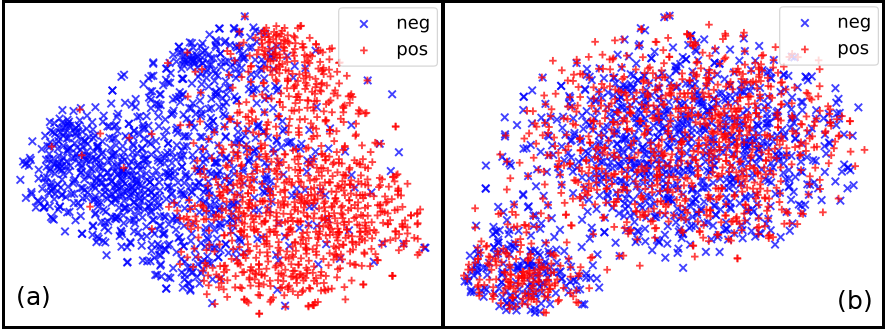
\includegraphics[width=\linewidth]{images/tsne-style-and-content}
	\caption{t-SNE plots of (a) style and (b) content spaces.}
	\label{fig:tsne}
\end{figure}


The latent space can be visualized with t-SNE plots~\cite{maaten2008visualizing} in Figure~\ref{fig:tsne}. As expected, sentences with different sentiments can be nicely separated in the style space (LHS), but are highly mixed in the content space (RHS).


\subsection{Style-Transfer Sentence Generation}

We apply the disentangled latent space to a style-transfer sentence generation task, where the goal is to generate a sentence with different sentiment (style). We followed \cite{fu2017style} and used two metrics: (1) For style transfer, we train a style classifier and predict the accuracy of the generated sentences. While the style classifier itself may not be perfect, it provides a quantitative way of evaluating the strength of style transfer. (2) For the content-preservation score, we compute a sentence embedding by min, max, and average pooling of word embeddings; then a cosine similarity is computed to evaluate how close two sentences are in meaning. Here, sentiment words from a stop list \cite{hu2004mining} are removed.

We compare our approach with state-of-the-art previous work in Table~\ref{tab:comparison-previous}. We re-conducted the experiments with their publicly available code on our data splits.
Results show that, our approach achieves a comparable content-preservation score with previous work, but a significantly better style-transfer score, showing that our disentangled latent space can be used for better style-transfer sentence generation.

Table~\ref{tab:ablation-results} presents the results of an ablation test. We see that both adversarial loss and reconstruction loss play a role in the strength of style transfer, and that they can be combined to further improve performance.

Some examples of style-transfer sentence generation are illustrated in Table~\ref{tab:transfer-samples}. We see that, with the empirically estimated style vector, we can flexibly control the sentiment of generated sentences.

\begin{table}[!t]
	\centering
	\begin{tabular}{| l | r | r | }
		\hline
		\textbf{Model}                       & \textbf{Style Transfer} & \textbf{Content Preservation} \\
		\hline
		\hline
		Cross-alignment \cite{shen2017style} & 0.4609                  & 0.8830                        \\
		\hline
		Sentiment embed. \cite{fu2017style}  & 0.4009                  & 0.9246                        \\
		\hline
		Ours                                 & 0.7708                  & 0.8958                        \\
		\hline
	\end{tabular}
	\caption{Comparison with previous approaches.}
	\label{tab:comparison-previous}
\end{table}

\begin{table}[!t]
	\centering
	\begin{tabular}{| l | r | r |}
		\hline
		\textbf{Training Loss}                          & \textbf{Style Transfer} & \textbf{Content Preservation} \\
		\hline
		\hline
		$J_\text{rec}$                                  & 0.5053                  & 0.9103                        \\
		\hline
		$J_\text{rec}$, $J_\text{adv}$                  & 0.5901                  & 0.9121                        \\
		\hline
		$J_\text{rec}$, $J_\text{mult}$                 & 0.6445                  & 0.9053                        \\
		\hline
		$J_\text{rec}$, $J_\text{adv}$, $J_\text{mult}$ & 0.7708                  & 0.8958                        \\
		\hline
	\end{tabular}
	\caption{Ablation test.}
	\label{tab:ablation-results}
\end{table}

\begin{table}[!t]
	\centering
	\begin{tabular}{| p{0.45\linewidth} | p{0.45\linewidth} |}
		\hline
		\textbf{{Original}}                                                        & \textbf{Transferred (Positive $\rightarrow$ Negative)}                    \\
		\hline
		\hline
		i bought this cuisipro mister to replace my old mister last june-(number)  & i bought this a couple of times and was disappointed in this product      \\
		\hline
		quality is good, recevied in time and works as expected.                   & quality is good but i am returning it                                     \\
		\hline
		all in all, i am very happy with this headset.                             & all in all i was expecting a good product                                 \\
		\hline
		\hline
		\textbf{{Original}}                                                        & \textbf{Transferred (Negative $\rightarrow$ Positive)}                    \\
		\hline
		\hline
		i sent it back and requested a refund, and never got the refund.           & i sent it back and gave it a try and it works great                       \\
		\hline
		so i tried just one (number) piece each n still the same results.          & so i bought the two sizes and the other ones are great                    \\
		\hline
		i am going to buy a replacement and wish i had sent this back for a refund & i am going to go through the same time and i have been using it for years \\
		\hline
	\end{tabular}
	\caption{Examples of style-transfer generation.}
	\label{tab:transfer-samples}
\end{table}


%======================================================================
\chapter{Experiments}
%======================================================================

\section{Evaluation Metrics}

\subsection{Cycle Loss}

Cycle loss is not a good metric because while transferring from $X$ to $Y$, and back to $X'$, the variable $Y$ is not observable and if the neural network function is accidentally fitted to transform the content domain, this metric will not be able to tell the difference between an over-fit model and a good model.


\section{Experiment Results}

We conducted experiments on an Amazon product review data-set, following \cite{fu2017style}. It contains 131072, 2048, 32768 sentences for train, validation, and test, respectively, each sampling accompanied by binary sentiment labels.

\subsection{Disentangling Latent Space}

We first analyze how the style (sentiment) and content of the latent space are disentangled. We train a logistic classifier based on different latent spaces, and show results in Table~\ref{tab:classification}.

We see that the 128-dimensional content vector is not discriminative for style. It achieves an accuracy of 0.57, slightly better than random/majority guess. However, the 8-dimensional style vector $\bm s$, despite its low dimensionality, achieves significantly higher style classification accuracy. When combining content and style vectors, we achieve no further improvement. These results verify the effectiveness of our disentangling approach, because the style space does contain style information, whereas the content space doesn't.


\begin{table}
	\centering
	\begin{tabular}{| l | r |}
		\hline
		Random/Majority guess           & 0.5000          \\ \hline
		Content latent space  ($\bm c$) & 0.5690          \\
		Style latent space ($\bm s$)    & \textbf{0.7817} \\
		Combined ($[\bm s;\bm c]$)      & 0.7815          \\
		\hline
	\end{tabular}
	\caption{Style classification accuracy.}
	\label{tab:classification}
\end{table}

\begin{figure}
	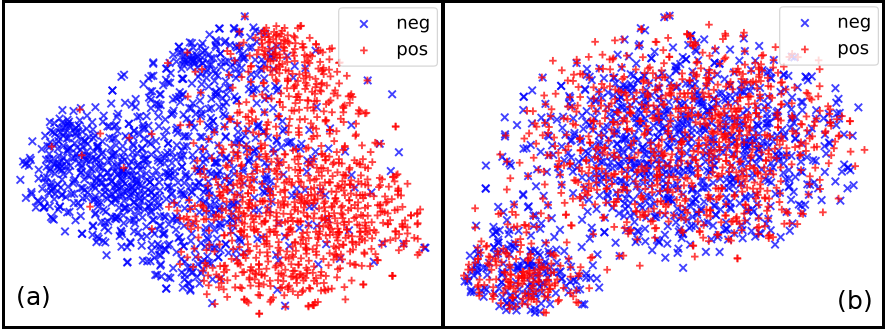
\includegraphics[width=\linewidth]{images/tsne-style-and-content}
	\caption{t-SNE plots of (a) style and (b) content spaces.}
	\label{fig:tsne}
\end{figure}


The latent space can be visualized with t-SNE plots~\cite{maaten2008visualizing} in Figure~\ref{fig:tsne}. As expected, sentences with different sentiments can be nicely separated in the style space (LHS), but are highly mixed in the content space (RHS).


\subsection{Style-Transfer Sentence Generation}

We apply the disentangled latent space to a style-transfer sentence generation task, where the goal is to generate a sentence with different sentiment (style). We followed \cite{fu2017style} and used two metrics: (1) For style transfer, we train a style classifier and predict the accuracy of the generated sentences. While the style classifier itself may not be perfect, it provides a quantitative way of evaluating the strength of style transfer. (2) For the content-preservation score, we compute a sentence embedding by min, max, and average pooling of word embeddings; then a cosine similarity is computed to evaluate how close two sentences are in meaning. Here, sentiment words from a stop list \cite{hu2004mining} are removed.

We compare our approach with state-of-the-art previous work in Table~\ref{tab:comparison-previous}. We re-conducted the experiments with their publicly available code on our data splits.
Results show that, our approach achieves a comparable content-preservation score with previous work, but a significantly better style-transfer score, showing that our disentangled latent space can be used for better style-transfer sentence generation.

Table~\ref{tab:ablation-results} presents the results of an ablation test. We see that both adversarial loss and reconstruction loss play a role in the strength of style transfer, and that they can be combined to further improve performance.

Some examples of style-transfer sentence generation are illustrated in Table~\ref{tab:transfer-samples}. We see that, with the empirically estimated style vector, we can flexibly control the sentiment of generated sentences.

\begin{table}[!t]
	\centering
	\begin{tabular}{| l | r | r | }
		\hline
		\textbf{Model}                       & \textbf{Style Transfer} & \textbf{Content Preservation} \\
		\hline
		\hline
		Cross-alignment \cite{shen2017style} & 0.4609                  & 0.8830                        \\
		\hline
		Sentiment embed. \cite{fu2017style}  & 0.4009                  & 0.9246                        \\
		\hline
		Ours                                 & 0.7708                  & 0.8958                        \\
		\hline
	\end{tabular}
	\caption{Comparison with previous approaches.}
	\label{tab:comparison-previous}
\end{table}

\begin{table}[!t]
	\centering
	\begin{tabular}{| l | r | r |}
		\hline
		\textbf{Training Loss}                          & \textbf{Style Transfer} & \textbf{Content Preservation} \\
		\hline
		\hline
		$J_\text{rec}$                                  & 0.5053                  & 0.9103                        \\
		\hline
		$J_\text{rec}$, $J_\text{adv}$                  & 0.5901                  & 0.9121                        \\
		\hline
		$J_\text{rec}$, $J_\text{mult}$                 & 0.6445                  & 0.9053                        \\
		\hline
		$J_\text{rec}$, $J_\text{adv}$, $J_\text{mult}$ & 0.7708                  & 0.8958                        \\
		\hline
	\end{tabular}
	\caption{Ablation test.}
	\label{tab:ablation-results}
\end{table}

\begin{table}[!t]
	\centering
	\begin{tabular}{| p{0.45\linewidth} | p{0.45\linewidth} |}
		\hline
		\textbf{{Original}}                                                        & \textbf{Transferred (Positive $\rightarrow$ Negative)}                    \\
		\hline
		\hline
		i bought this cuisipro mister to replace my old mister last june-(number)  & i bought this a couple of times and was disappointed in this product      \\
		\hline
		quality is good, recevied in time and works as expected.                   & quality is good but i am returning it                                     \\
		\hline
		all in all, i am very happy with this headset.                             & all in all i was expecting a good product                                 \\
		\hline
		\hline
		\textbf{{Original}}                                                        & \textbf{Transferred (Negative $\rightarrow$ Positive)}                    \\
		\hline
		\hline
		i sent it back and requested a refund, and never got the refund.           & i sent it back and gave it a try and it works great                       \\
		\hline
		so i tried just one (number) piece each n still the same results.          & so i bought the two sizes and the other ones are great                    \\
		\hline
		i am going to buy a replacement and wish i had sent this back for a refund & i am going to go through the same time and i have been using it for years \\
		\hline
	\end{tabular}
	\caption{Examples of style-transfer generation.}
	\label{tab:transfer-samples}
\end{table}


%----------------------------------------------------------------------
% END MATERIAL
%----------------------------------------------------------------------

% B I B L I O G R A P H Y
% -----------------------

% The following statement selects the style to use for references.  It controls the sort order of the entries in the bibliography and also the formatting for the in-text labels.
\bibliographystyle{unsrtnat}
% This specifies the location of the file containing the bibliographic information.  
% It assumes you're using BibTeX (if not, why not?).
\cleardoublepage % This is needed if the book class is used, to place the anchor in the correct page,
% because the bibliography will start on its own page.
% Use \clearpage instead if the document class uses the "oneside" argument
\phantomsection  % With hyperref package, enables hyperlinking from the table of contents to bibliography             
% The following statement causes the title "References" to be used for the bibliography section:
\renewcommand*{\bibname}{References}

% Add the References to the Table of Contents
\addcontentsline{toc}{chapter}{\textbf{References}}

\bibliography{uw-ethesis}
% Tip 5: You can create multiple .bib files to organize your references. 
% Just list them all in the \bibliogaphy command, separated by commas (no spaces).

% The following statement causes the specified references to be added to the bibliography% even if they were not 
% cited in the text. The asterisk is a wildcard that causes all entries in the bibliographic database to be included (optional).
\nocite{*}

\end{document}
